\documentclass{article}
\usepackage[table]{xcolor}
\usepackage{fullpage}
\usepackage{tabularx}
\usepackage{graphicx}
\usepackage{amsmath}
\usepackage{hyperref}
\usepackage{listings}
\lstset{frame=single, language=python, tabsize=4}
\usepackage{tikz}
\usetikzlibrary{arrows.meta,automata,quotes,positioning,babel}
\usetikzlibrary{shapes.geometric, arrows}

\begin{document}
	\title{Deep Learning Approaches to Graph mining}
	\author{Yuchen Hou}
	\maketitle

\section{Introduction}
Both academia and industry have seen pervasive adoption of deep learning since early 2010s,
when they began to outperform other machine learning techniques in various 
application domains, e.g.,
speech recognition \cite{hannun2014deep},
image recognition \cite{simonyan2014very},
natural language processing \cite{yao2013recurrent},
recommendation systems \cite{barkan2016item2vec},
and graph mining \cite{grovernode2vec}.
Deep learning can not only achieve higher prediction accuracy than other methods,
but also require much less domain knowledge and engineering.

Among those domains,
graph mining is a new and active application area for deep learning.
As neural nets have demonstrated their power in many domains,
we naturally wonder if we can apply them in prediction problems in graph mining,
and what kind of techniques are helpful in using their power.

My intended PhD research is deep learning approaches to graph mining.
Specifically, I investigate deep learning approaches to
two important types of problems in graph mining:
\begin{itemize}
	\item Predicting node and link attributes, e.g., boolean and numeric node attributes, link existence and link weight.
	\item Predicting graph attributes, e.g., the security status of a computer network and the chemical activity of a compound.
\end{itemize}

\section{Background}
The research in graph mining has advanced many fields
where objects and their relations can be modeled by nodes and links in a network, e.g.,
computer networks \cite{bermond1995distributed},
social networks \cite{cook2006mining},
protein interaction networks \cite{bader2003automated},
ecological food webs \cite{brown2003ecological},
and citation networks \cite{greenberg2009citation}.

An important problem in graph mining is link prediction \cite{liben2007link},
e.g., to predict whether a person will follow another person in a social network.
Link existence prediction is a well-known problem,
but one of its related problems is not: link weight prediction.
To be more specific,
the link prediction problem actually refers to link existence prediction:
to predict whether a link from a node to another node exists or will form.
Link weight prediction is
to predict the weight of a link from a node to another node
so the question it cares about is not if two nodes are connected,
but how likely or how strong they are connected.
This consideration is very practical in many scenarios.
For example, when describing a connection in a social network,
to say Alice likes Bob is not as precise as
to say Alice texts/tweets/mentions Bob 128 times per day on average,
because the second description is quantitative and more informative.
A special case of link weight prediction is collaborative filtering.
For example, to predict users' ratings to movies
is to predict the link weights on the bipartite graph
where the two disjoint node sets are users and movies.

Another important problem is graph classification \cite{duda2012pattern}.
More specifically, it is to the prediction of whether a graph has a label,
i.e., to predict a boolean attribute.
This problem has extremely high value in many fields.
For example, in pharmaceutical industry,
to predict whether a compound causes a certain disease
can be modeled as to predict whether a graph representing the compound
has the label of the disease.

\section{Preliminary research}
In our preliminary research,
we want to create a technique to predict link weights in a graph.
The estimator we need should learn to represent the graph in a meaningful way
and to learn to predict the target link weights using that representation.

\subsection{Problem}
We consider the problem of link weight prediction in a weighted directed graph.
We first take a look at an example of the problem,
and then give the problem a definition.
An undirected graph can be reduced to a directed graph by converting each weighted undirected link to two directed links with the same weight and opposite directions,
so the prediction for a weighted undirected graph is a special case of the problem we consider.

\subsubsection{Problem example}
Let us look at an example of link weight prediction - message volume prediction in a social network, shown in \autoref{fig:example} and \autoref{tab:example}.
In this example, there are 3 users in a social network: A, B and C.
Each user can send any amount of text messages to every other user.
We know the message size transmitted between A and C, B and C, but not A and B.
We want to predict the message size transmitted between A and B.
\begin{figure}[!htb]\centering
	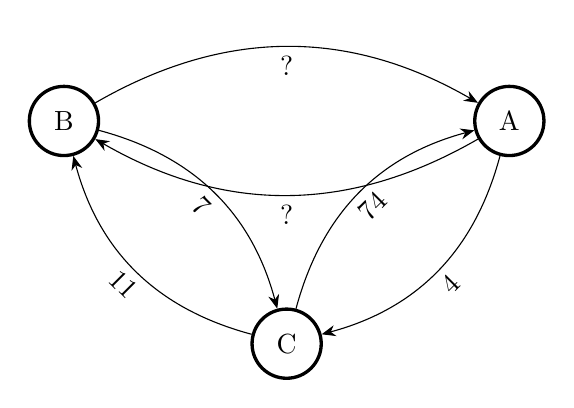
\begin{tikzpicture}[
	node distance = 4cm,
	on grid,
	> = {Stealth[length=5pt,width=4pt]},
	every state/.style = {very thick},
	every edge quotes/.style = {sloped, anchor=north}
	]
	\node[state] (B) {B};
	\node[state] (C) [below right=of B] {C};
	\node[state] (A) [above right=of C] {A};
	\path[->]   
	(A) edge[bend left,"?"]   (B)
	(B) edge[bend left,"7"]   (C)
	(B) edge[bend left,"?"]   (A)
	(A) edge[bend left,"4"]   (C)
	(C) edge[bend left,"74"]  (A)
	(C) edge[bend left,"11"]  (B);
	\end{tikzpicture}
	\caption{
		An example of link weight prediction in a weighted directed graph -
		message volume prediction in a social network.
		There are 3 users - A, B and C - in this network.
		Each user can send any amount of text messages to every other user.
		Here is what we know:
		A sent 4 messages to C,
		B sent 7 messages to C,
		and C sent 74 and 11 messages to A and B.
		What we do not know and what we want to predict is
		the message volume A and B sent to each other.
		}
	\label{fig:example}
\end{figure}
\begin{table}[!htb]\centering
	\caption{
		The same example as \autoref{fig:example}, but with edge list representation for the network.
	}
	\begin{tabularx}{0.6\textwidth}{|X|X|c|}  \hline \rowcolor{blue!40}
		Source node & Destination node & Link weight \\ \hline
		A & B & ? \\ \hline
		A & C & 74 \\ \hline
		B & A & ? \\ \hline
		B & C & 7 \\ \hline
		C & A & 4 \\ \hline
		C & B & 11 \\ \hline
	\end{tabularx}
	\label{tab:example}
\end{table}
This is a simplified network similar to many real social networks, where every user interacts with other users by posting, sharing, following or liking them.
There can not be any logical approach to derive the unknown message volumes,
as they have randomness.
But there can be statistical approaches to build models to predict them.
The ability to predict these interactions potentially allows us to recommend new connections to users:
if A is predicted/expected to send a large amount of messages to B by some model,
and A is not connected to B yet,
we can recommend B as a new connection to A.

\subsubsection{Problem definition}
Now we define the link weight prediction problem in a weighted directed graph.
\begin{itemize}
	\item Given a weighted directed graph with the node set V and link subset E
	\item Build a model w = f(x, y) where x and y are nodes and w is the weight of link (x, y) that can predict the weight of any link
\end{itemize}
There is one thing to clarify about this definition.
For every possible link (1 out of $ n^2 $, where n is the number of nodes), 
if we know its weight, we know it exists;
if we do not know its weight, we do not know it exists.
This is a very practical point when we handle streaming graphs:
for any possible link,
we either know it exists and know its weight (if it has been streamed in), or we do not know if the link will ever exist, nor know its weight.

\subsection{Related work}
In our literature study on previous research,
we have found existing approaches to the link weight prediction problem
and deep learning approaches to problems related to link weight prediction problem,
but no deep learning approaches to link weight prediction problem.
In this section, we review these existing approaches.

\subsubsection{SBM (Stochastic Block Model) approach to link weight prediction}
This approach is designed for unweighted graphs and uses only link existence information \cite{holland1983stochastic}.
The main idea is to partition nodes into L groups and connect groups with bundles.
In this way, the graph has a 2-level structure:
\begin{itemize}
	\item Lower level: each group consists of nodes which were topologically similar in the original graph
	\item Upper level: groups are connected by bundles
	to represent the original graph
\end{itemize}
Given a graph with adjacency matrix A, the SBM has the following parameters:
\begin{itemize}
	\item A: link existence matrix, where $ A_{ij} \in \{0, 1\} $
	\item z: the group vector,
	where $ z_i \in \{ 1 ... L \} $ is the group label of node i
	\item $ \theta $: the bundle existence probability matrix,
	where $ \theta_{z_i z_j} $ is the existence probability of bundle ($z_i, z_j$)
\end{itemize}
So the existence of link (i, j) $ A_{ij} $ is a binary random variable following the Bernoulli distribution:
\begin{align*}
	A_{ij} \sim B(1, \theta_{z_i z_j})
\end{align*}
The SBM fits parameters z and $ \theta $
to maximize the probability of observation A:
\begin{align*}
	P(A|z, \theta) 
	= \prod_{ij} \theta_{z_i z_j}^{A_{ij}}(1-\theta_{z_i z_j})^{1-A_{ij}}
\end{align*}
The SBM has a few derivatives designed for weighted graphs
that use link weight information,
including pWSBM (pure Weighted Stochastic Block Model),
bWSBM (balanced Weighted Stochastic Block Model and
DCWBM (Degree Corrected Weighted Stochastic Block Model) \cite{aicher2014learning}.

\subsubsection{Deep learning approaches to problems related to link weight prediction}
There are a few deep learning approaches to
the node classification problem (i.e., to predict whether a node has a label) and 
link existence prediction problem (i.e., to predict whether a link exists).
Two earlier approaches are graph neural nets and relational neural 
nets \cite{scarselli2009graph},
where neural nets are incorporated into a traditional iterative graph 
information propagation approach.
A newer approach is deep walk \cite{perozzi2014deepwalk}, 
where a graph is reduced to a natural language corpus so that existing neural 
net model designed for natural language processing - skip-gram model - can handle the graph.
A very recent approach is node2vec \cite{grovernode2vec},
which uses the same skip-gram model, 
but a different way to reduce the graph to a natural language corpus.
The word2vec technique is famous for using a neural net to learn to map every 
entity (word in this case) in a vocabulary to a vector without any domain 
knowledge \cite{mikolov2013efficient}.
The subsequent techniques item2vec \cite{barkan2016item2vec}
and node2vec \cite{grovernode2vec} use the same skip-gram 
model used in word2vec to map items and nodes to vectors.
In a corpus, every word is described/defined only by related words in its 
contexts, by implicit relations between words in word co-occurrences.
Nonetheless, the neural net can learn from word co-occurrences and map words to 
vectors accordingly,
such that the relations between words are preserved in the word vector space 
\cite{mikolov2013distributed}.
The same arguments apply to relations between items and between nodes.

\subsection{Deep learning approach}
We build an estimator with a neural net model using a node pair as its input
and the weight of the link connecting the nodes as its output.

\subsubsection{Model R}
We design the model in the estimator as a fully connected neural net which we call Model R (R as in "relation"), shown in Figure \ref{fig:model}.
We have considered a convolutional neural net as an alternative,
but there is no spacial property in the input node vectors
for a convolutional neural to take advantage of,
compared to the 2D array of an image where the spacial location of each pixel
has significant meaning (e.g., relative distances of pixels).

\begin{figure*}[!htb]
	\centering
	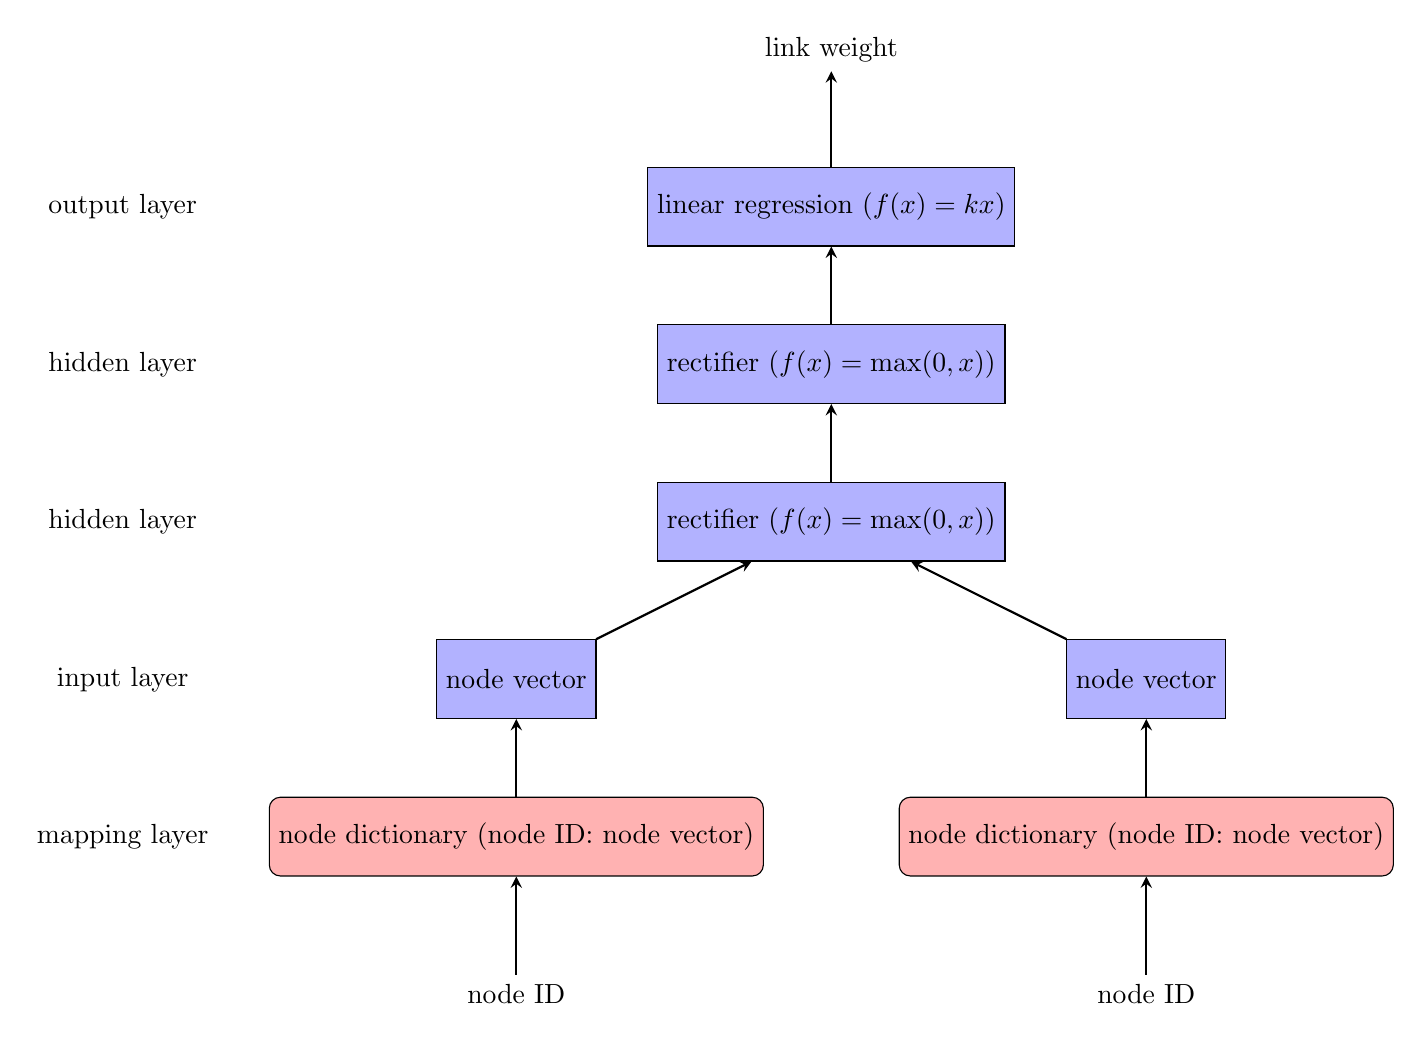
\begin{tikzpicture}[node distance=2cm]
	\tikzstyle{startstop} = [rectangle, rounded corners, minimum width=1cm, 
	minimum height=1cm, text centered, draw=black, fill=red!30]
	\tikzstyle{process} = [rectangle, minimum width=1cm, minimum height=1cm, 
	text centered, draw=black, fill=blue!30]
	\tikzstyle{arrow} = [thick,->,>=stealth]
	\node (linearRegression) [process] {linear regression ($ f(x) = kx $)};
	\node (relu0) [process, below of=linearRegression] {rectifier ($ f(x) = \max (0, x) $)};
	\node (relu) [process, below of=relu0] {rectifier ($ f(x) = \max (0, x) $)};
	\node (linear1) [process, below of=relu, xshift=-4cm] {node vector};
	\node (linear2) [process, below of=relu, xshift=4cm] {node vector};
	\node (oneHot1) [startstop, below of=linear1] {node dictionary (node ID: node vector)};
	\node (oneHot2) [startstop, below of=linear2] {node dictionary (node ID: node vector)};
	\node (weight) [above of=linearRegression] {link weight};
	\node (output) [left of=linearRegression, xshift=-7cm] {output layer};
	\node (hidden0) [below of=output] {hidden layer};
	\node (hidden) [below of=hidden0] {hidden layer};
	\node (input) [below of=hidden] {input layer};
	\node (mapping) [below of=input] {mapping layer};
	\node (source) [below of=oneHot1] {node ID};
	\node (destination) [below of=oneHot2] {node ID};
	\draw [arrow] (source) -- (oneHot1);
	\draw [arrow] (destination) -- (oneHot2);
	\draw [arrow] (oneHot1) -- (linear1);
	\draw [arrow] (oneHot2) -- (linear2);
	\draw [arrow] (linear1) -- (relu);
	\draw [arrow] (linear2) -- (relu);
	\draw [arrow] (relu0) -- (linearRegression);
	\draw [arrow] (relu) -- (relu0);
	\draw [arrow] (linearRegression) -- (weight);
	\end{tikzpicture}
	\caption{
		Model R for a weighted graph.
		Only layers and their connections are shown,
		while the units in each layer and their connections are not shown.
		We feed every node to the estimator by feeding the ID.
		During learning,
		the estimator learns and populates the vectors in the tables.
	}
	\label{fig:model}
\end{figure*}
The model contains the following layers:
\begin{itemize}
	\item A mapping layer that maps node IDs to node vectors.
	In the node dictionary,	the key is the node ID, the value is the node vector,
	which is learned through back propagation and stochastic gradient descent.
	\item An input layer directly activated by the node dictionaries.
	Its activations are the two node vectors.
	\item Multiple fully connected hidden layers of rectified linear units
	(only two layers are shown in the figure).
	These units employ the rectifier ($ f(x) = \max (0, x) $)
	as their activation function.
	Compared to earlier popular activation functions like sigmoid function
	($ f(x) = (1 + \exp(-x))^{-1} $),
	rectifier not only simplifies and accelerates computation,
	but also eliminates vanishing gradient problems,
	and has become the most popular activation function
	for deep neural networks \cite{lecun2015deep}.
	These layers learn to extract more and more abstract weight-relevant 
	information.
	\item An output layer with a linear regression unit.
	This unit employs linear regression ($ f(x) = kx $) as its activation function.
	It learns to predict the link weight as a real number
	using abstracted weight-relevant information.
\end{itemize}
Link weights provide the information about nodes.
We fully take this property into account and design this model to learn 
complex and unobservable node information (i.e., node vectors) 
supervised by a simple and observable relations between nodes (i.e., link weight).

\subsubsection{Learning techniques}
The estimator uses the above model and a number of popular deep learning 
techniques:
\begin{itemize}
	\item Backpropagation: propagation of the error gradients from output layer 
	back to each earlier layer \cite{rumelhart1988learning}
	\item Stochastic gradient descent: the optimization that minimizes 
	the error (descending against the error gradient in weight space) for a 
	random sample in each gradient descent step \cite{lecun2012efficient}
	\item Mini-batch: the modification to stochastic gradient descent to 
	accelerate and smooth the descent by minimizing the error for a small 
	random batch of samples in each gradient descent step \cite{mairal2010online}
	\item Early stopping: the regularization used to reduce over-fitting during the iterative learning process by stopping the learning when validation error stops decreasing \cite{smale2007learning}
\end{itemize}

\subsection{Experiments}
We evaluate Model R experimentally with SBM, pWSBM, bWSBM and DCWBM as baselines,
and compare their prediction errors on several datasets.
We use the same datasets and experiment process used in a recent study of these baselines \cite{aicher2014learning}.
The results show 
that Model R can achieve much lower prediction error than the baseline models.

\subsubsection{Datasets}
The experiments use four datasets summarized in \autoref{tab:datasets}.
\begin{table*}[!htb]\centering
	\caption{The datasets used in experiments.}
	\begin{tabularx}{\textwidth}{|c|c|X|c|X|}  \hline \rowcolor{blue!40}
		Dataset & Node count & Node type & Link count & Link weight type \\ \hline
		Airport\cite{colizza2007reaction} & 500 & busiest airports in US & 5960 & number of passengers traveling from one airport to the other\\ \hline
		Collaboration\cite{pan2012world} & 226 & nations on Earth & 20616 & number of academic papers written by authors from the two connected nations \\ \hline
		Congress\cite{porter2005network} & 163  & 102nd US Congress committees & 26569 & interlock value of shared members from the two committees \\ \hline
		Forum\cite{opsahl2009clustering}  & 1899 & users of a student social network at UC Irvine & 20291 & number of messages sent from one student to the other \\ \hline
	\end{tabularx}
	\label{tab:datasets}
\end{table*}

\subsubsection{Experiment results}
In our experiments,
Model R's error is lower than every other model on every dataset,
shown in \autoref{fig:errors}.
\begin{figure*}[!htb]\centering
	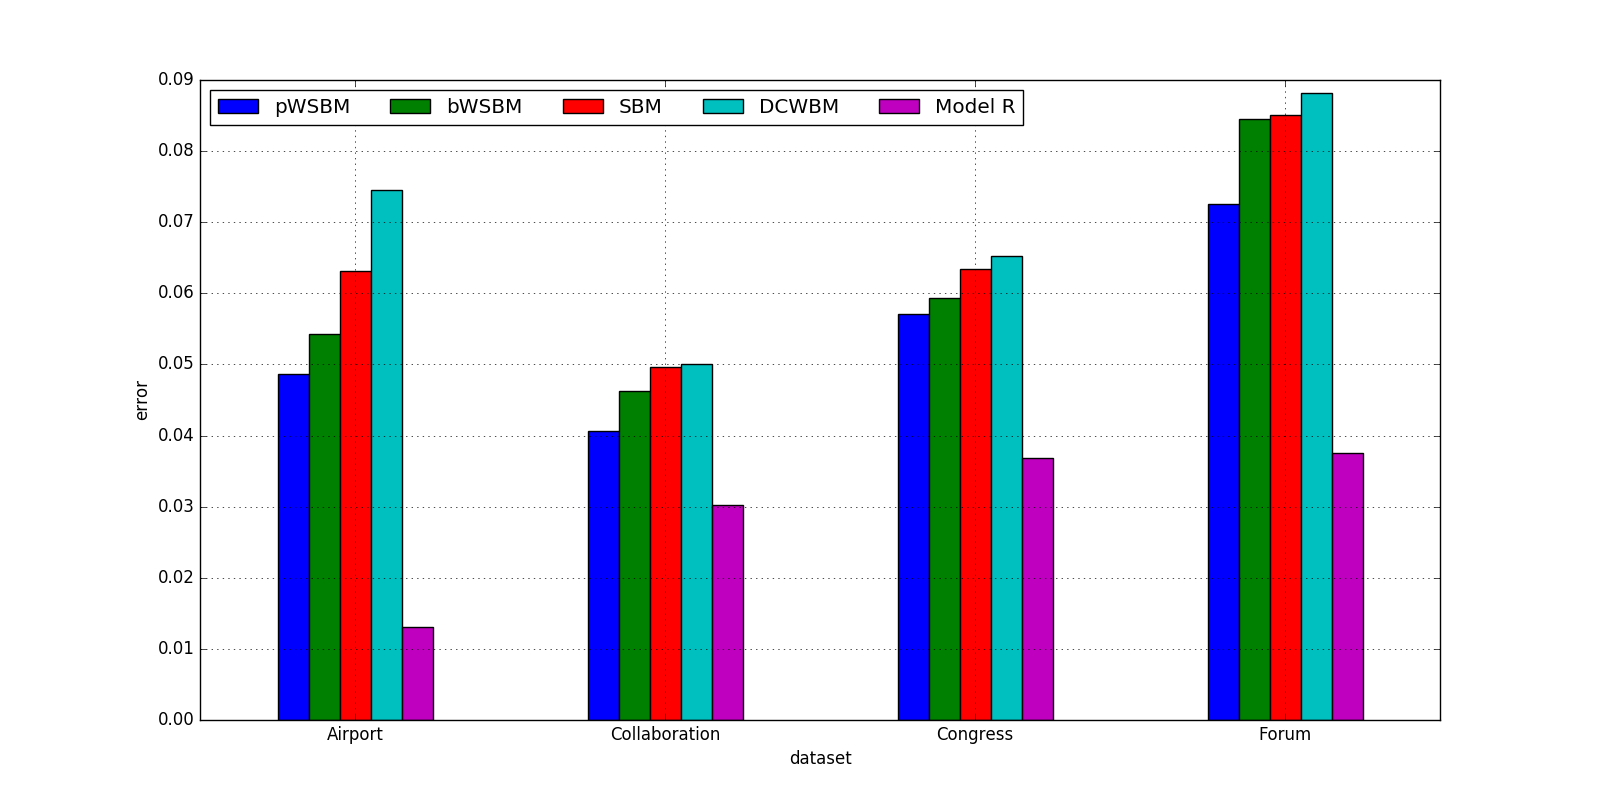
\includegraphics[width=\textwidth]{link-weight-errors}
	\caption{
		The mean squared errors of 5 models on 4 datasets:
		Model R has lower error than every other model on every dataset.
		Every error value shown here is the mean errors for the 25 trials in the experiment.
	}
	\label{fig:errors}
\end{figure*}
In this section we compare Model R with the baseline models on every dataset.
Given the dataset,
we regard ModelRError (as well as BaselineError) as a random variable
so each trial generates an example of it.
We can do a Student's t-test to justify the significance of difference between the means of variables ModelRError and BaselineError.
The mean of a variable is not the same as the mean of a sample of the variable.
More specifically, a variable can generate two samples with different sample means,
therefore two samples with different means do not imply the two variables generating them have different means.
For each dataset, we do a t-test for the two variables where the null hypothesis is that the two variables have the same mean:
\begin{align*}
\overline{ModelRError} = \overline{BaselineError}
\end{align*}
where $ \overline{X} $ is the mean of variable X.
The smaller p value is in the t-test, the more confidently we can reject the null hypothesis, i.e., accept that:
\begin{align*}
\overline{ModelRError} \neq \overline{BaselineError}
\end{align*}
Typically there is a domain specific threshold for p, e.g., 0.1 or 0.01. If p is smaller than the threshold we reject the null hypothesis.
We calculate the p value and also error reduction from baseline to Model R as:
\begin{align*}
Reduction = \frac{BaselineError - ModelRError}{BaselineError}
\end{align*}
The p value is almost 0 for all datasets and error reduction is significant,
shown in \autoref{tab:errors}.
Model R has lower error than every other model on every dataset,
reducing error by 25\% to 73\% from the best baseline model - pWSBM.
The number in every parenthesis is the standard deviation of the errors in 25 trials in the last digit. The very low p values strongly indicate the error reduction is significant.
\begin{table*}[!htb]\centering
	\caption{
		The mean squared errors with standard deviations of 5 models on 4 datasets.
	}
	\begin{tabularx}{\textwidth}{|c|X|X|X|X|X|c|c|} \hline \rowcolor{blue!40}
		Dataset & pWSBM & bWSBM & SBM & DCWBM & Model R & Reduction & p \\ \hline
		Airport & 0.0486 $ \pm $ 0.0006 & 0.0543 $ \pm $ 0.0005 & 0.0632 $ \pm $ 0.0008 & 0.0746 $ \pm $ 0.0009 & 0.013 $ \pm $ 0.001 & 73\% & 4.2e-66 \\ \hline
		Collaboration & 0.0407 $ \pm $ 0.0001 & 0.0462 $ \pm $ 0.0001 & 0.0497 $ \pm $ 0.0003 & 0.0500 $ \pm $ 0.0002 & 0.030 $ \pm $ 0.001 & 25\% & 9.1e-44 \\ \hline
		Congress & 0.0571 $ \pm $ 0.0004 & 0.0594 $ \pm $ 0.0004 & 0.0634 $ \pm $ 0.0006 & 0.0653 $ \pm $ 0.0004 & 0.036 $ \pm $ 0.003 & 35\% & 7.1e-35 \\ \hline
		Forum & 0.0726 $ \pm $ 0.0003 & 0.0845 $ \pm $ 0.0003 & 0.0851 $ \pm $ 0.0004 & 0.0882 $ \pm $ 0.0004 & 0.037 $ \pm $ 0.001 & 48\% & 4.2e-68 \\ \hline
	\end{tabularx}
	\label{tab:errors}
\end{table*}
These results show that Model R outperforms pWSBM on all these datasets.

\subsection{Conclusion}
Model R shows that deep learning can be successfully applied to link weight prediction problem.
It effectively learns complex and unobservable node information (i.e., node vectors) from simple and observable relations between nodes (i.e., link weight),
and uses that information to predict unknown link weights.
Compared to Stochastic Block Model based approaches,
this neural net model is much more accurate.
We anticipate this new approach will provide effective solutions to more
graph mining problems.

\subsection{Papers}
\begin{enumerate}
	\item Rejected: ASONAM 2017, Node mapping: Link attribute prediction with neural networks
	\item Rejected, resubmission planned: AAAI 2017, Deep Learning Approach to Collaborative Rating Prediction
	\item In review: IJCNN 2017, Deep Learning Approach to Link Weight Prediction
\end{enumerate}

\section{Future research}
In our future research,
we want to study deep learning approaches to graph attribute prediction problem.
The estimator we need should learn to represent the graph in a meaningful way
and to learn to predict the target graph attribute using that representation.

\subsection{Problem}
We consider the graph attribute prediction problem
in a graph where nodes and links have attributes.
This attribute can be boolean (classification) or numeric (regression).
For simplicity, we focus on classification problem only.
We first take a look at an example of the problem,
and then give the problem a definition.
Later we will discuss how to handle graph regression problem.

\subsubsection{Problem example}
Let us look at an example of graph attribute prediction problem - compound activity prediction shown in \autoref{fig:protein}.
In this problem, the estimator needs to learn to predict the compound activity
based on the compound structure.
More specifically, we show the estimator the training set of examples,
where the input is the graph representing the compound structure and
the output is the compound activity.
And the estimator needs to predict the unknown activity of each compound
in the testing set.
In general, the activity is a vector
where each element represents a specific type of activity.
\begin{figure*}[!htb]\centering
	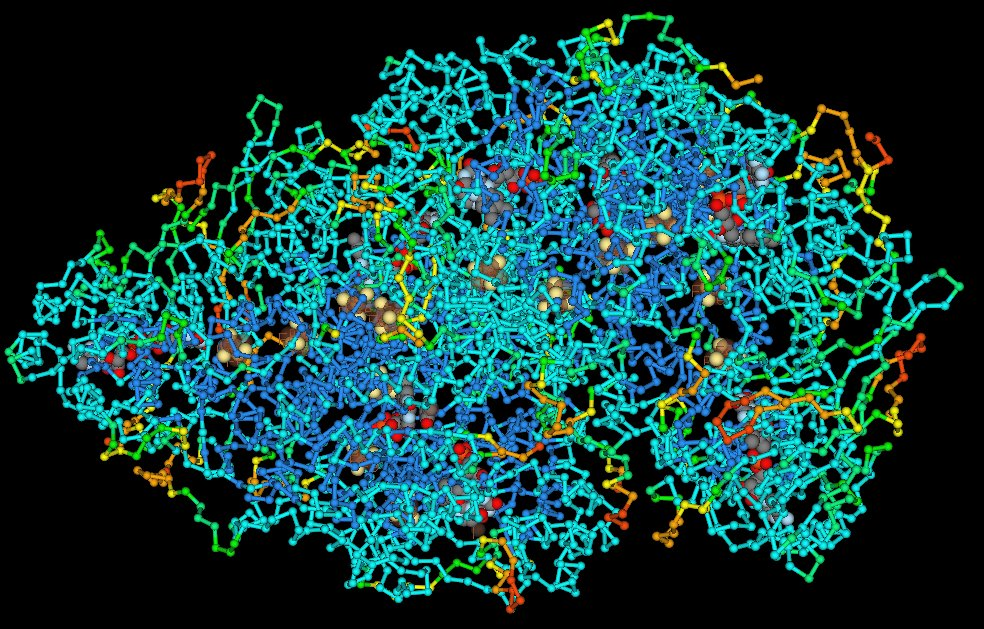
\includegraphics[width=\textwidth]{ProteinStructure}
	\caption{
		The chemical structure of a polypeptide macromolecule:
		Nodes and links in this graph represent atoms and bonds in the compound,
		where attributes (colors) of the nodes and links represents
		the types of the atoms and bonds.
		A polypeptide is a linear organic polymer consisting of a large number of amino-acid residues bonded together in a chain.
		However, in general, a compound can have any topology.
	}
	\label{fig:protein}
\end{figure*}

\subsubsection{Problem definition}
Now we define the graph attribute prediction problem in an undirected graph.
\begin{itemize}
	\item Given a set of undirected graphs, where each graph has a known target attribute and every node and link has one attribute.
	\item Build a model y = f(x) where x is the graph and y is the target attribute of x, that can predict the target attribute of any graph.
\end{itemize}

\subsection{Related work}
In our literature study on previous research,
we have found existing approaches to graph classification problem
and deep learning approaches to problems related to graph classification problem,
but no deep learning approaches to graph classification problem.
In this section, we review these existing approaches.

\subsubsection{Graph kernel approach to graph classification}
This approach is similarity based \cite{kashima2003marginalized}.
The model is similar to support vector machines:
\[ y = f(x) = \sum_{i} \alpha_i K(x, x_i) \]
where the sign of y is the target attribute, f is the model,
x is the testing example, $ \alpha_i $'s are target attribute levels',
$ x_i $'s are training examples, and
$ K(x, x_i) $ is the label sequence graph kernel
that measures the similarity of x and $ x_i $.
In the training stage,
the model learns an $ \alpha_i $ for each $ x_i $;
in prediction stage,
it predicts y as 
the sum of $ \alpha_i $ weighted by $ K(x, x_i) $'s \cite{scholkopf2001learning}.

An example kernel function is the label sequence graph kernel,
based on graph paths,
where each path is represented by the sequence of attributes of the nodes and links
on the path.
For example, in the graph shown in \autoref{fig:example},
we can represent a path from node A to node B via node C as (A, 4, C, 11, B).
In this example, the node attributes are categorical and link attributes are numeric.
In general, the node attributes and link attributes appear alternatively.
The label sequence graph kernel is defined as
\[ K(x_1, x_2) =
\sum_{h_1 \in x_1} \sum_{h_2 \in x_2} 
k(h_1, h_2) p(H = h_1 | x_1) p(H = h_2 | x_2) \]
where $ x_1, x_2 $ are two graphs,
$ h_i $ is any path in $ x_i $,
$ k(h_1, h_2) $ is the label sequence path kernel
that measures the similarity of $ h_1, h_2 $,
H is a random path variable predefined by a random walking policy W, and
$ p(h_i | x_i) $ is the conditional probability of $ H = h_i $ given $ x_i $.
There are many implementations for W and k.
An example W can be, at any node:
\begin{itemize}
	\item stop the walk with probability c (constant)
	\item walk to any neighbor with probability $ (1 - c) / D $,
	where D is the degree of the node
\end{itemize}
An example k can be Kronecker delta: 1 when the two paths are the same and 0 otherwise.
The model calculates $ K(x_1, x_2) $ as
the sum of $ k(h_1, h_2) $ weighted by $ p(H = h_1 | x_1) p(H = h_2 | x_2) $.

\subsubsection{Graph boosting approach to graph classification}
This approach is feature based \cite{saigo2009gboost}.
It requires feature engineering with domain knowledge.
For example, in chemistry informatics, experts can define a set of discriminative chemical substructures as the features.
And a compound can be represented by a feature vector where each element indicates
the presence of a certain substructure.
In general, this approach needs a predefined set of subgraphs and convert the
graph to a feature vector where each element is the presence or count of a certain subgraph.
With this feature vector, standard machine learning models (including neural network models) can learn to predict the target attribute with this feature vector.
Many recent claims of deep learning approaches to compound activity prediction
take this approach by applying neural network as the machine learning model
\cite{unterthiner2015toxicity}, \cite{unterthiner2014deep} \cite{ramsundar2015massively}.
In this research, we do not consider them as real deep learning approaches,
because they involve feature engineering with domain knowledge.

\subsubsection{Image recognition approach to graph classification}
This approach takes advantage of the advancement of deep learning in image recognition by converting a graph to an image and apply standard deep learning techniques developed for image recognition \cite{wallach2015atomnet}.
This approach requires the nodes in the graph to have explicit coordinates -
instead of only the topologies - e.g., the atom coordinates in a compound.
The coordinates allow the construction of a 3D image of the compound,
shown in \autoref{fig:protein}.
In this research, we do not consider it as a deep learning approach to real
graph classification problem because it requires nodes to have locations.

\subsection{Observations and possible deep learning approaches to graph classification}
Now we review make observations about those existing approaches and
propose possible deep learning approaches to graph classification inspired by them.

\subsubsection{Graph kernel inspired deep learning approach}
Path sequences of node and link attributes in a graph is similar to
sentences of characters in a natural language document.
So a potential approach is to reduce a graph to a document and apply deep learning techniques developed for natural language processing.
The neural net for this approach can be either recurrent or convolutional.

\subsubsection{Graph boosting inspired deep learning approach}
Subgraphs in a graph are similar to sub-images in an image.
If, instead of counting those predefined subgraphs,
we use deep learning to learn to detect and examine all discriminative subgraphs,
we may get a end to end deep learning approach for graph classification.
We haven't seen deep learning techniques developed for this process,
but we've found previous research on eye movement \footnote{https://en.wikipedia.org/wiki/Eye\_movement}
providing evidences that humans examine images using
saccade (macro movement of gaze from a sub-image to another sub-image)
\footnote{https://en.wikipedia.org/wiki/Saccade} and
fixation (micro movement of gaze within a sub-image)
\footnote{https://en.wikipedia.org/wiki/Fixation\_(visual)}.
Human visual system is shown to be able to detect and examine all discriminative
sub-images in a sequence and comprehend the image.
Therefore, a potential approach to graph classification is
to directly detect and examine all discriminative subgraphs in a sequence.
Examining subgraphs can be easier because the size of a subgraph is bounded,
while that of a graph is not.
However, it is not clear if there are other ways to represent a subgraph
except sampling paths in the graph as in graph kernel.
The neural net for this approach needs memory so it should be recurrent.
It might also have convolutional neural net when examining every subgraph.
There is one significant difficulty in this approach:
although a sub-image (e.g., a face in a person)
almost always exists in a image dataset,
a sub-graph (e.g., a substructure of a compound)
might not always exists in a compound dataset.
Another difficulty is subgraph examination might be just as hard as graph classification.
One last difficulty is that the movement between two subgraphs may
require complex policy from reinforcement learning or search strategy.

\bibliographystyle{IEEEtran}
\bibliography{references}
\end{document}
